\documentclass[11pt]{report}
\usepackage{StyleSheets/main}
\begin{document}

\chapter{System Risk Management}\label{ch:system-risk-management}
The purpose of this section is to manage the possible risks of this system. Possible risks will be identified, and solutions for risk mitigation will be brought forward. This section is an important way for the team to be prepared for any possible setbacks and to limit the amount of setbacks taken in an effort for the project to run smoothly.

\begin{figure}[H]
    \centering
    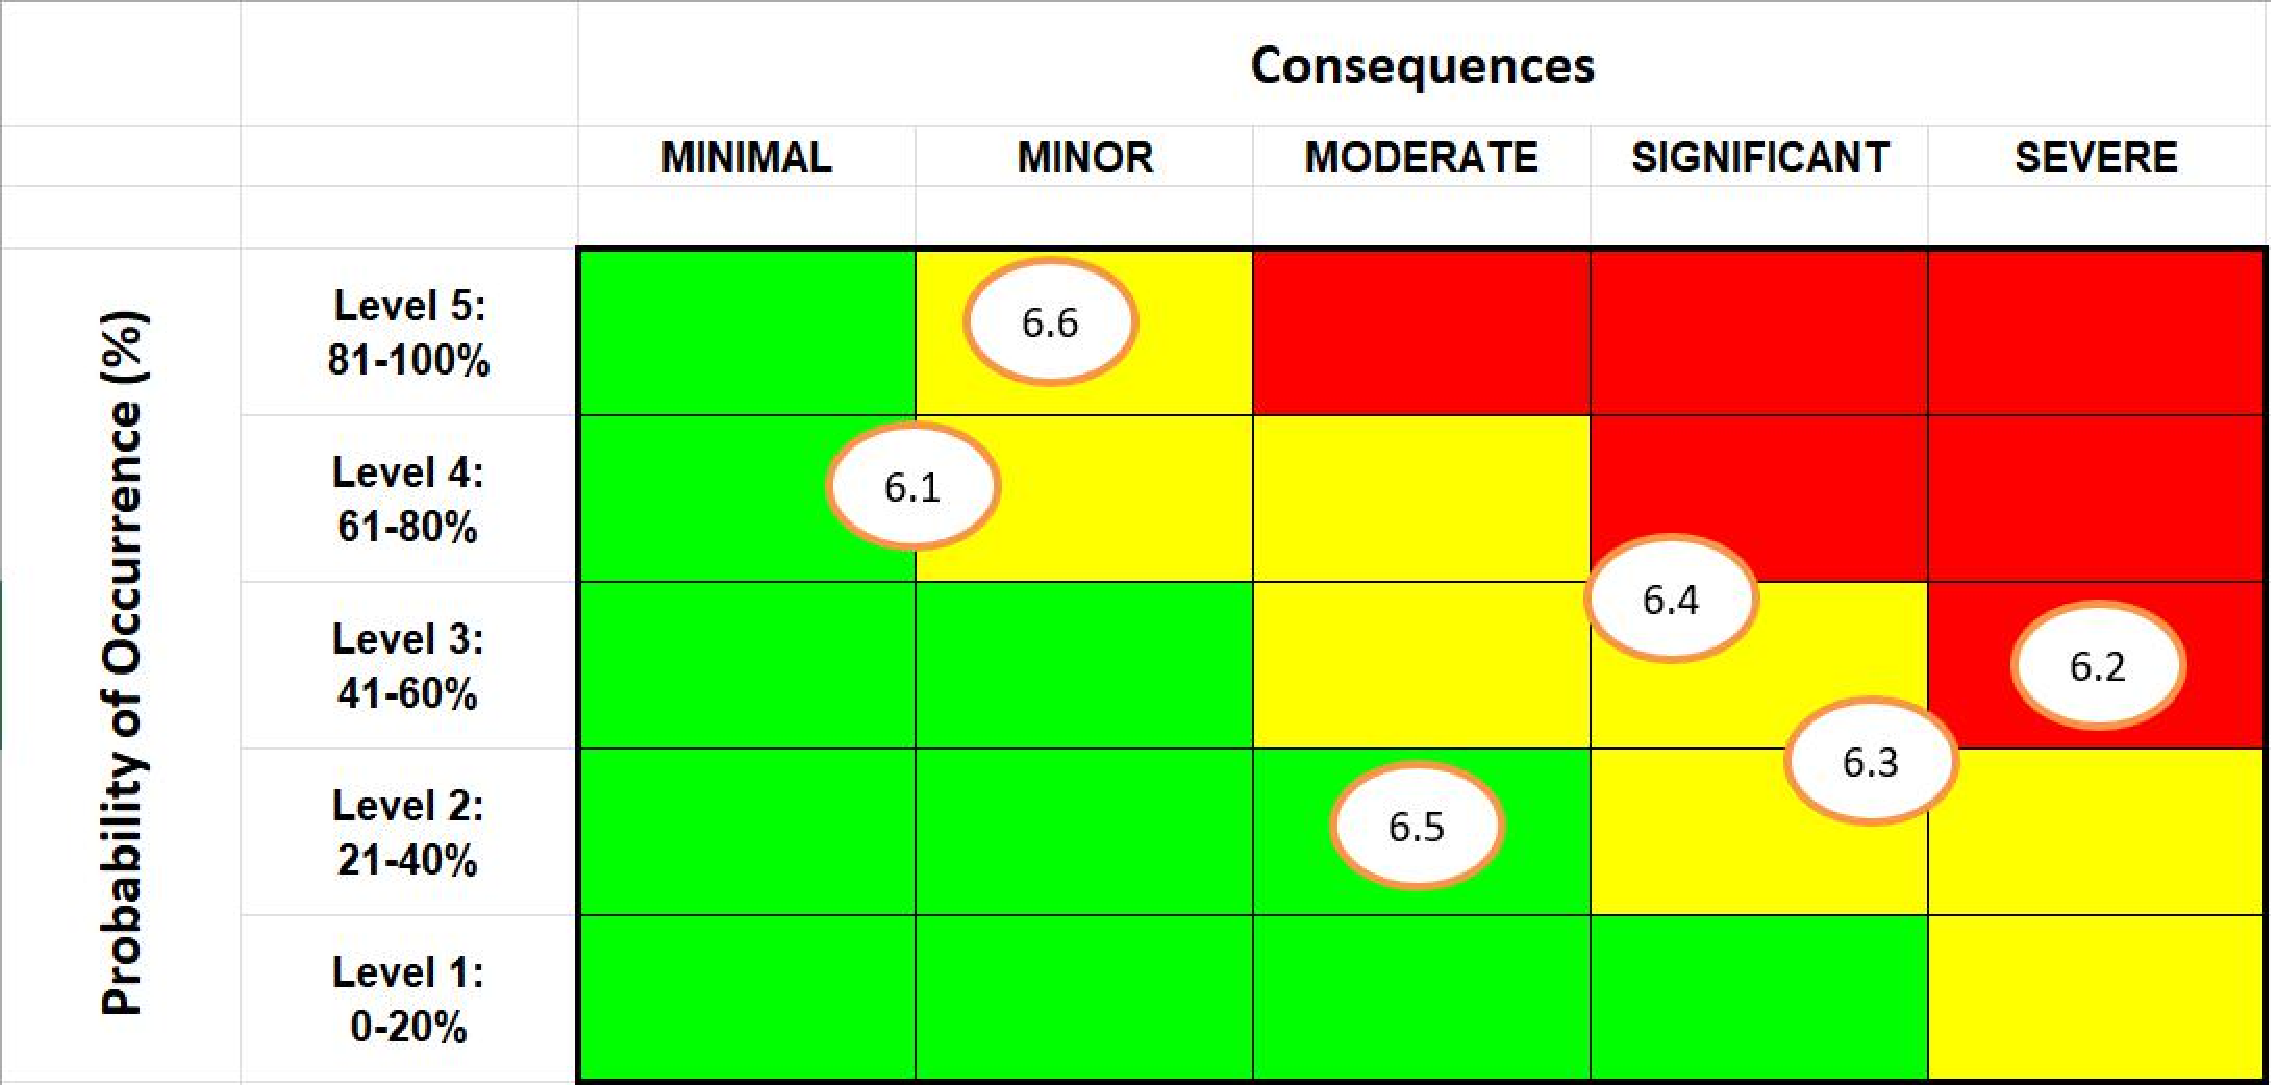
\includegraphics[width=0.8\linewidth]{Graphs/SystemRiskManagementGraph.pdf}
    \caption{System Risk Management Assessment Chart}
    \label{fig:system-management}
\end{figure}

\section{Failure of 3D Prints during printing}
\begin{itemize}
    \item Risk: This system required a lot of 3D prints for sensor mounts and vehicle structure. It is possible that during printing these prints fail due to the nature of 3D printing. 
    \item Mitigation: If multiple of the same print are printed at a time, the risk of a print failing is greatly reduced. Introducing redundancy into 3D prints is a great way to lose the uncertainty of a print failing. For example, if a sensor mount has enough space on the printing board for 2 or even 3 prints, the maximum amount of prints should be done just in case of the event of failure. 
\end{itemize}
\section{Burning of an Electrical Feature}
\begin{itemize}
    \item Risk: During robot testing, it is possible for a wire to be misplaced or a mistake to be made resulting in an electrical feature in the robot heating up, burning, and possible becoming permanently damaged. Electrical features in this system which are at risk of this issue are the Teensy 4.1 microcontroller, the motor controllers, and the \gls{DC}--\gls{DC} converters. This can also become a risk to the operator of the vehicle, as it could result in an electrical fire or the operator getting hurt or injured.
    \item Mitigation: In the event of an electrical part burning, a new part can be bought, however it is better for this not to be the case. When handling voltages which are capable of destroying sensitive parts, care must be taken to avoid the damage of these parts. Before operation of the vehicle, make certain that the wiring matches the diagram seen in \cref{fig:Pinoutmap}. If the robot is switched on and no lights turn on, there may be a short, and should be immediately turned off and troubleshooted.
\end{itemize}
\section{Failure or Breaking of a Motor} 
\begin{itemize}
    \item Risk: During testing of the robot, it is possible that a motor becomes incorrectly placed or incorrectly wired. This can result in damage to the motor, which is a massive risk to the system.
    \item Mitigation: While a new motor can be bought for the system, it is better to avoid this as it is out of budget. When handling the motor, it is essential that the motor is handled and installed with care. 
\end{itemize}
\section{Damage to Parts During Soldering}
\begin{itemize}
    \item Risk: During soldering of parts of the vehicle, it is possible that the soldering iron can burn parts of the robot. The temperatures which are being dealt with during soldering are very high and would break any part which is made contact with. 
    \item Mitigation: During soldering of wires and parts, extreme care must be taken to not damage the parts of the vehicle. Care must be taken to ensure that the soldering iron does not come in contact with the motor or other easily damaged electrical parts of the vehicle.
\end{itemize}
\section{Running out of Budget for the System}
\begin{itemize}
    \item Risk: It is a risk that the budget for the system is exceeded. This can limit the changes which are made to the vehicle due to the lack of funds available. 
    \item Mitigation: Cost saving measures should be taken throughout the project. Attempting to save as much money from the budget as possible is essential, while care must be taken to not cut corners and induce other failures.
\end{itemize}
\section{Lack of Correspondence of Color Sensors}
\begin{itemize}
    \item Risk: With past experience and knowledge of the color sensors used in this system, it is known that the color sensors are very difficult to work with and are very sensitive to external light or shiny surfaces.
    \item Mitigation: It is important to not let the color sensors be affected by external light. This can be done by introducing ``curtains'' around the color sensors to ensure that the only light which is seen by them is their own light. Reducing the amount of variables around the color sensors is important in ensuring their accuracy. It is also important to calibrate the colors and surfaces on which the vehicle will be running to reduce the sensitivity of the system to shiny or reflective surfaces. 
\end{itemize}
\end{document}
